\section{Idée commerciale}
LoRaSnow est une solution autonome de détection de hauteur de neige. 
Il arrive parfois que les routes mettent du temps à être déneigées, ou que le salage soit trop
faible, conduisant à une chaussée glissante et dangereuse. De plus, une répartition inhomogène du manteau neigeux sur une
région peut rendre la tâche compliquée, surtout en montagne. LoRaSnow apporte un monitoring constant
des niveaux de neige sur la route et du débit de neige à des points clés ainsi que les possibilités de verglas.\\[0.2cm]
Grâce à un réseau de capteurs sur une région, il devient possible d’optimiser la courses des chasses-neige
et de cibler les axes en plus grandes difficultés, de même que d’offrir l’opportunité d’effectuer des sa-
lages préventifs, avant que du verglas ne se forme.\\[0.2cm]
Se présentant sous forme d'abonnement annuel, il suffit au client de souscrire et de bénéficier
d'un service de surveillance des routes. Le client n'aura pas à ce soucier d'éventuels pannes, installations
et infrastructures, tout est compris dans l'abonnement.

\section{Domaine d'activité}
Le domaine d'activité principal est la détection de hauteur de neige sur route de montagne.

\section{Marché}
Des communes, comme Ayent, ont manifesté leur intérêt pour une solution
de détection du niveau de neige sur route.
Des entreprises privées de déneigement bénéficieraient de LoRaSnow pour
optimiser leur service de déneigement et améliorer la qualité du service
fourni.\\
Pour lancer le produit, il faudra d'abord cibler les communes avec stations de ski,
qui ont plus de moyen et de raison de ce tourner vers l'innovation.\newpage

\section{Analyse des risques}
\begin{figure}[H]
    \centering
    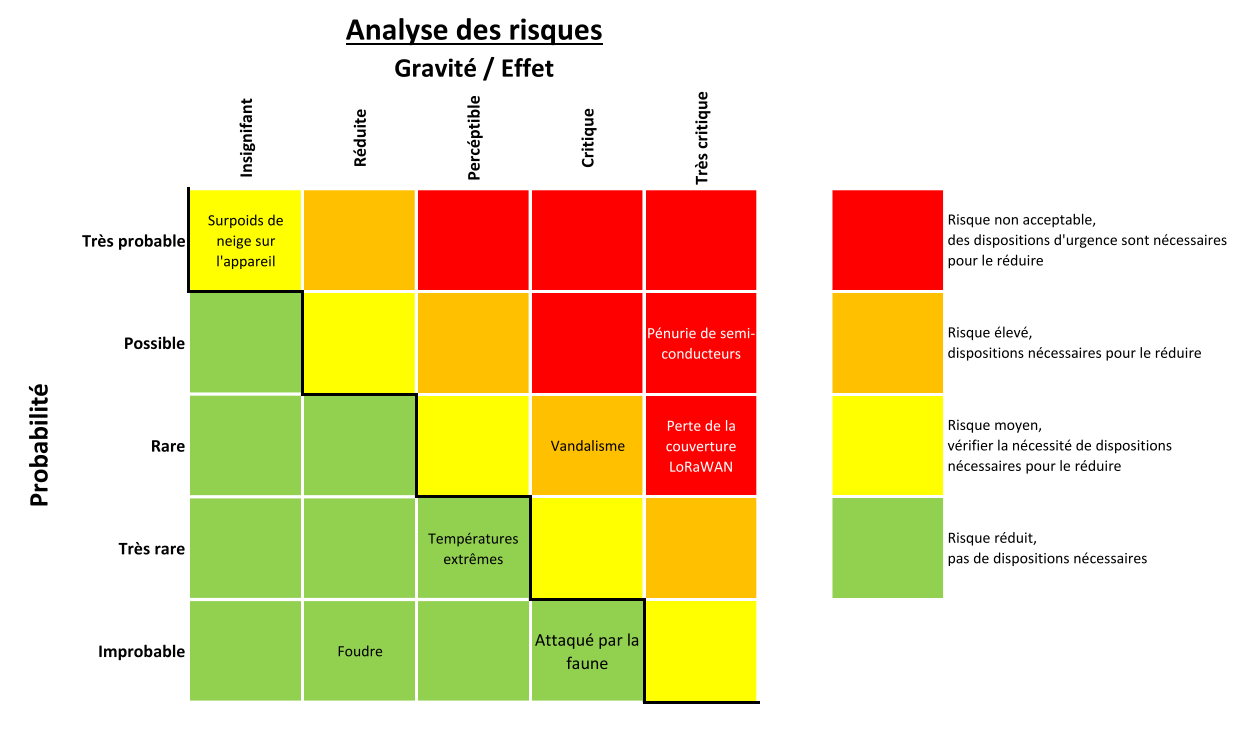
\includegraphics[width=\linewidth]{Images/business/risiko.PNG}
    \caption[]{Analyse des risques}
    \label{fig:risiko}
\end{figure}

Il est possible qu'une installation soit endommagée ou détruite par la faune, l'environnement
ou par un simple vandale. Les causes naturels sont trop improbables pour être considérées.
Le vandalisme sera paré par des installations très discrète: afin d'éviter que les automobilistes
s'arrêtent, pensant qu'il s'agit d'un nouveau radar de la police et le vandalisant en conscéquence.
Une assurance est également à prévoir si une installation discrète n'est pas possible.\\[0.2cm]
L'appareil étant prévu pour effectuer des mesures sous la neige, il va inévitablement se trouver couvert
d'une grande couche de neige. La casquette du boitier permet d'éviter l'enneigement de la vitre et
le montage du boitier est suffisamment solides pour supporter de fortes charges. Rendant ce risque insignifiant.\\[0.2cm]
Il faut prévoir une redondance pour le réseau LoRaWAN. On est pas à l'abri d'une panne de gateway, et si cela arrive
tous les appareils dans la nature ne pourrait plus transmettre leurs données. Il faut donc toujours avoir 3 appareils
qui couvrent une région pour éviter une perte de couverture.\\[0.2cm]
La pénurie de semi-conducteur persiste et pourrait persister encore longtemps. Pour éviter de se retrouver à
ne pas pouvoir respecter les commandes des clients, il pourrait être préférable d'attendre quelques années avant
d'envisager l'industrialisation et commercilisation du projet.